\documentclass[11pt, oneside]{article} 
\usepackage{geometry}
\geometry{letterpaper} 
\usepackage{graphicx}
	
\usepackage{amssymb}
\usepackage{amsmath}
\usepackage{parskip}
\usepackage{color}
\usepackage{hyperref}

\graphicspath{{/Users/telliott_admin/Tex/png/}}
% \begin{center} 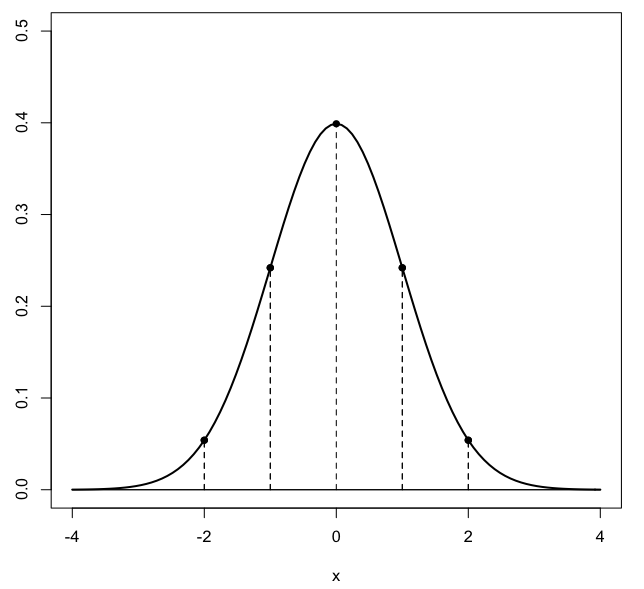
\includegraphics [scale=0.4] {gauss3.png} \end{center}

\title{Taylor series}
\date{}

\begin{document}
\maketitle
\Large

Suppose we have a function $f(x)$, but 

Shankar:

\begin{quote}"imagine that you don't have access to the whole function.  You cannot see the whole thing.  You can only zero-in on a tiny region."\end{quote}

around $f(0)$, where you know the value.  So the question is, what do we guess the function will do near $f(0)$?  
 
The first approximation is that
\[ f(x) \approx f(0) \]
We really can't say anything more.  $f(0)$ is the best guess for what the value of the function is (we're talking about continuous and continuously differentiable functions).

Now suppose we know the slope of the function at $0$, $f'(0)$.  Then, since 
\[ \Delta y = f'(0) \Delta x = f'(0) (x - 0) \]
we can get a better approximation as the linear approximation:
\[ f(x) \approx f(0) + f'(0)\ x + \dots \]

For most functions, there will be more terms.  If $f$ is not a linear function, then the slope won't be constant.  So 

\begin{quote}"the rate of change itself has a rate of change .. the second derivative."\end{quote}  

The term we are going to add is
\[ f''(0)\ \frac{x^2}{2} \]
so
\[ f(x) \approx f(0) + f'(0)\ x + f''(0)\ \frac{x^2}{2}  + \dots \]

A simple way to see why we have $x^2/2$ is to take derivatives on both sides.  The terms like $f'(0)$ and $f''(0)$ are constants, they have been evaluated at $x=0$. The first derivative is
\[ f'(x) \approx  f'(0) + f''(0)\ x  + \dots \]
We evaluate at $x=0$ and the term $f''(0)\ x$ goes away because of the $x=0$ multiplying the constant $f''(0)$.  So we have just
\[ f'(x) \approx  f'(0)  \]
and that matches. Now take the second derivative
\[ f''(x) \approx  f''(0) \]
and that matches too.  We can see a pattern here.  

The fourth term is
\[ f(x) \approx f(0) + f'(0)\ x + f''(0)\ \frac{x^2}{2!}  + f'''(0)\ \frac{x^3}{3!} + \dots \]

You might not be expecting the factorial which I snuck in there.  But if you go back to the exercise above, where we evaluated derivatives, you can see why it works.  When we take the first derivative 
\[ \frac{d}{dx} (f'''(0)\ \frac{x^3}{3!}) =  f'''(0)\ \frac{x^2}{2!}\]
the $3$ comes down from the power and then turns $3!$ in the denominator into $2!$.  The next derivative will bring down the $2$.  So everything cancels properly.  

If you like $\Sigma$ notation, we can write
\[ f(x) = \sum_{n=0}^{\infty} f^n(0) \frac{x^n}{n!} \]
with the understanding that $0! = 1$.  The approximation is better the closer $x$ is to $0$, and the more terms the better as well.  

There is one final wrinkle to this derivation.  The series can be modified deal with $x$ near any value $a$, not just near $0$.  The modification is
\[ f(x) = \sum_{n=0}^{\infty} f^n(a) \frac{(x-a)^n}{n!} \]
This is the Taylor series.  The series near $a=0$ is known as the Maclaurin series.

\subsection*{1/1-x}
The first example is
\[ f(x) = \frac{1}{1-x} \]
We know the answer to this.
\[ \frac{1}{1-x} = 1 + x + x^2 + x^3 \]
Proof:
\[ 1 = (1-x)(1 + x + x^2 + x^3) \]
Multiplying by $1$, the second term $x$ is matched by $-x$ from the first term in the multiplication by $-x$, and so on.  The whole thing vanishes, leaving just $1$.

We want to evaluate $f(x)$ near $0$, let's say, at $x=0.1$.  The correct value of the function is
\[ f(x) = \frac{1}{0.9} = 1.11111 \dots \]

Let's try to approximate using the series.  We need derivatives
\[ f(x) = \frac{1}{1-x} \]
\[ f'(x) = \frac{1}{(1-x)^2} = (1-x)^{-2} \]
\[ f'(0) = 1 \]
so the linear approximation is
\[ f(x) \approx 1 + 1x = 1.1 \]

For the next term we obtain
\[ f''(x) = 2(1-x)^{-3} \]
The $2$ is cancelled by the $2!$ in the denominator, so this cofactor is $1$ and we're left with
\[ f''(0)\ \frac{x^2}{2} = x^2 = 0.01 \]
And I think we can see where this one is going.

However, you probably remember that this series
\[ \frac{1}{1 - x} = 1 + x + x^2 + x^3 + \dots \]
diverges for $|x| \ge 1$, and the Taylor series does too.

The morale of the story is that for some series, there is a radius of convergence and the series is only valid for $x$ within that radius.

\subsection*{binomial}\

Another very useful series is the binomial.
\[ f(x) = (1 + x)^n \]
\[ f(0) = 1 \]
\[ f'(0) = n(1 + x)^{n-1} = n \]
\[ f''(0) = n(n-1)(1 + x)^{n-2} = n(n-1) \]
So the series is
\[ (1 + x)^n \approx 1 + nx + n(n-1) \frac{x^2}{2} \]

We use this one a lot.

A nice application is relativistic energy
\[ E = mc^2 f \]
\[ f =  1/\sqrt{1-\frac{v^2}{c^2}} \]
This is, in disguise, a binomial with $n=-1/2$ and $x=-v^2/c^2$ so the expansion is
\[ f  \approx 1 + nx = 1 + \frac{v^2}{2c^2} \]
so the energy is 
\[ E \approx mc^2 (1 + \frac{v^2}{2c^2} ) \]
And we see that the second term is just the kinetic energy, $mv^2/2$.

\subsection*{polynomials}

The beauty of Taylor Series (despite its complexity) is that it turns any differentiable function into a polynomial.  Polynomials are easy to integrate and work with.

The first thing to say about Taylor Series is they give the correct answer for functions that we know.  For example, suppose we have 
\[ f(x) = ax^2 + bx + c = 1 \]
We get the derivatives and evaluate them "near" the point $x=0$.
\[ f(x) = ax^2 + bx + c = c \]
\[ f'(x) = 2ax + b = b \]
\[ f''(x) = 2a \]
The series is then
\[ f(x) = c + b(x) + \frac{21}{2!}(x)^2 + \cdots \]
But there are no more terms.  That's it.  And this is just
\[ f(x) = c + bx + ax^2 \]

\subsection*{exponential, sine and cosine}

Suppose $f(x) = e^x$ and again, we evaluate "near" $x=0$.  We have
\[ f(x) = e^x = 1 \]
\[ f'(x) = e^x = 1 \]
\[ f''(x) = e^x = 1 \]
The series is
\[ f(x) = e^x = f(0) + \frac{f'(0)}{1!}(x-0) + \frac{f''(0)}{2!}(x-0)^2 + \frac{f'''(0)}{3!}(x-0)^3 + \cdots \]
\[ f(x) = 1 + \frac{1}{1!}x + \frac{1}{2!}x^2 + \frac{1}{3!}x^3 + \cdots \]
\[ f(x) = 1 + x + \frac{x^2}{2!} + \frac{x^3}{3!} + \cdots \]
Which matches what we already know about $e^x$.  For example, it is obvious that 
\[ \frac{d}{dx}e^x = e^x \]

Let's try to find something new.  Suppose we expand $f(x) = cos\ x$ near $x=0$
\[ f(x) = cos \ x = cos \ 0 = 1 \]
\[ f'(x) = -sin \ x = -sin \ 0 = 0 \]
\[ f''(x) =  -cos \ x -cos \ 0 = -1 \]
\[ f'''(x) =  sin \ x = sin \ 0 = 0 \]
\[ f''''(x) =  cos \ x =  cos \ 0 = 1 \]
and this continues in a cycle with period 4.
The series is
\[ f(x) = f(a) + \frac{f'(a)}{1!}(x-a) + \frac{f''(a)}{2!}(x-a)^2 + \frac{f'''(a)}{3!}(x-a)^3 + \cdots \]
\[ f(x) = cos \ x = 1 - \frac{1}{2!}(x-0)^2 + \frac{1}{4!}(x-0)^4 + \cdots \]
\[ f(x) = cos \ x = 1 - \frac{x^2}{2!} + \frac{x^4}{4!} + \cdots \]

Similarly, for $f(x) = sin \ x$ near $x=0$
\[ f(x) = sin \ x = 0 \]
\[ f'(x) = cos \ x = 1 \]
\[ f''(x) = -sin \ x = 0 \]
\[ f'''(x) =  -cos \ x = -1 \]
\[ f''''(x) =  sin \ x = 0 \]
The series is
\[ f(x) = f(a) + \frac{f'(a)}{1!}(x-a) + \frac{f''(a)}{2!}(x-a)^2 + \frac{f'''(a)}{3!}(x-a)^3 + \cdots \]
\[ f(x) = sin \ x = x - \frac{1}{3!}(x-0)^3 + \frac{1}{5!}(x-0)^5 + \cdots \]
\[ f(x) = sin \ x = x - \frac{x^3}{3!} + \frac{x^5}{5!} + \cdots \]

\subsection*{funny series}

In Strogatz book (\emph{The Joy of x}), he gives the following series
\[ 1 - \frac{1}{2} + \frac{1}{3} - \frac{1}{4} + \frac{1}{5} - \cdots \]
and he says that the sum of the series is equal to the natural logarithm of $2$:
\[ \ln 2 = 1 - \frac{1}{2} + \frac{1}{3} - \frac{1}{4} + \frac{1}{5} - \cdots \]
with the provision that you have to calculate the sum in the order given.

For example, the second, third and fourth partial sums are:
\[ S_2 = \frac{1}{2} ; \ \  S_3 = \frac{5}{6}; \ \ S_4 = \frac{14}{24}; \ \ S_5 = \frac{94}{120} \]
with $S_4 = 0.583$ and $S_5 = 0.783$.  For any partial sum $S_n$ and the previous sum $S_{n-1}$ the value of the series will be bounded by the two sums.

I thought I would try to show that $\ln 2$ is the correct value for series, by using a Taylor series for the logarithm.  

Taylor says we can write a function $f(x)$ (near the value $x=a$) as an infinite sum
\[ f(x) = \sum_{n=0}^\infty \frac{f^n(a)}{n!} (x-a)^n\]
where $f^n$ means the nth derivative of $f$ and $f^0$ is just $f$, and these derivatives are to be evaluated at $x=a$.
Near $a=0$ this simplifies to 
\[ f(x) = \sum_{n=0}^\infty \frac{f^n(0)}{n!} (x)^n\]

Let's calculate the derivatives of the logarithm:
\[ f^0 = \ln x; \ \ f^1 = \frac{1}{x} = x^{-1}; \ \ f^2 = -x^{-2}; \ \ f^3 = 2x^{-3}; \ \ f^4 = -3!\ x^{-4}  \]
The first thing I notice is that we can't use $a=0$, since $f^1 = 1/x$ is undefined there.  So, let's try $a=1$.  Then (evaluated at $a=1$)
\[ f^0 = \ln x = 0; \ \ f^1 = \frac{1}{x} = 1; \ \ f^2 = -x^{-2} = -1; \ \ f^3 = 2; \ \ f^4 = -3!  \]

Going back to the definition
\[ f(x) = \sum_{n=0}^\infty \frac{f^n(a)}{n!} (x-a)^n\]
I get the following series near $a = 1$:
\[ \ln x = \frac{0}{0!} (x-1)^0 +  \frac{1}{1!} (x-1)^1 - \frac{1}{2!} (x-1)^2 + \frac{2}{3!} (x-1)^3 - \frac{3!}{4!} (x-1)^4 + \cdots \]
For the special value $x=2$, all the terms $(x-1)^n$ go away (which confirms that $a=1$ is an excellent choice!).  We have then
\[ \ln x = \frac{0}{0!} +  \frac{1}{1!} - \frac{1}{2!} + \frac{2}{3!} - \frac{3!}{4!} + \cdots \]
\[ =  0 + 1 - \frac{1}{2} + \frac{1}{3} - \frac{1}{4} + \cdots \]
which is what was to be proved.

\end{document}  